\section{Stability and closures}\label{sec:closure}

\subsection{Instability of fitted network feedback}
The fitted models are evaluated above on the observed paths, where the network is sparse: on average only \DataWithinContacts\ contacts within classes exist at a time.
Simulated forward from an empty network with the timetable of a held-out day, every model with network context (M2, M3, M5) behaves differently: within minutes, contacts form faster than they end, and the network becomes dense (Fig.~\ref{fig:closure}).
The same happens when common contacts raise the attempt rate additively instead of the probability units (a variant with linear instead of exponential triadic closure, whose held-out likelihood is close to that of M2).
The reason is a positive feedback that the likelihood does not constrain: each common contact and each further current contact raises the formation rate, in the observed sparse states moderately, but without bound as groups grow, and the stabilizing effect of common contacts on termination adds to it.
Models without network context (M1, M4, M6, C1) are stable.
This is a form of model degeneracy, analogous to the degeneracy of exponential random graph models with triangle terms \citep{schweinberger2011}: the fitted parameters describe the observed configurations, but the process they define concentrates on configurations that are never observed.

\subsection{Simple and pair closure}
Mean-field equations generated from the rules can anticipate such behavior without simulation, but only if the closure keeps the correlations that drive it.
We compare two closures for the contacts within classes of the fitted M2 (\WithinClassShare\% of all contacts), treating each class as a homogeneous block whose pairs differ by their static marks (Facebook and survey friendship).
The \emph{simple closure} takes the numbers of common contacts and other contacts of a pair as Poisson variables with means given by the current density, independently of whether the pair is in contact.
The \emph{pair closure} adds as state variables the sums $Z$ and $O$ of the common contacts over pairs in contact ($Z$ = three times the number of triangles) and over pairs not in contact (open two-paths); given the state of a pair, its common contacts are Poisson with mean $Z/L$ or $O/U$ ($L$, $U$ the numbers of pairs in and not in contact), and the excess degrees follow from the degree moments implied by $Z + O$, the number of two-paths (App.~\ref{app:closure}).
Both closures have the same dense stationary state of about \DenseWithinContacts\ contacts within classes, but they reach it at very different times (Fig.~\ref{fig:closure}): the pair closure tips after about \PairTipMinutes\ minutes, close to the simulation (about \SimTipMinutes\ minutes), the simple closure only after about \SimpleTipMinutes\ minutes.
Triadic feedback acts through the correlation between a pair's state and its common contacts, which the simple closure discards; the pair closure keeps it, and with it the time scale of the instability.

\begin{figure}[t]
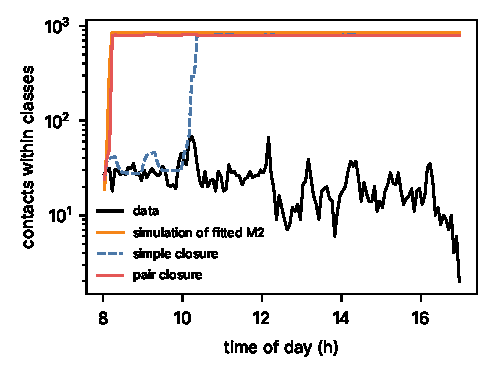
\includegraphics[width=\columnwidth]{generated/fig-closure}
\caption{Contacts within classes over a held-out day: data, simulations of the fitted network-context model M2 (mean of three runs, stopped when the network had become dense), and the simple and pair closures of the same model, all started from an empty network at 8:00 with the timetable as forced events.}
\label{fig:closure}
\end{figure}
